F\documentclass[11pt, a4paper, spanish, openright, twoside]{book}
\usepackage[spanish, activeacute]{babel}
\usepackage[utf8]{inputenc}
%\usepackage[top=2.5cm, bottom=2.5cm, outer=1.75cm, inner=1.75cm, heightrounded, marginparwidth=2.5cm, marginparsep=0.3cm]{geometry}	%márgenes empequeñecidos
\usepackage[top=2.95cm, bottom=2.25cm, outer=2.75cm, inner=2.75cm, heightrounded, marginparwidth=2.5cm, marginparsep=0.3cm]{geometry}	%márgenes originalmente
\usepackage{dpg}
\usepackage{fli}

\usepackage{pgf}
\usepackage{tikz}

\usepgflibrary{shapes.geometric} % LATEX and plain TEX and pure pgf
\usetikzlibrary{arrows,automata,positioning}
\tikzstyle{accepting by double}= [double distance=1.6pt,double,outer sep=.5\pgflinewidth+.8pt] % esto es algo estético.
\renewcommand\shorthandsspanish{}  % para compatibilizar spanish con tikz

%%%%%%		Figuras		%%%%%%%%%%%%%%%%%%%
\usepackage[vflt]{floatflt}		%Entorno float-figure

%%%%%%		Page style		%%%%%%%%%%%%%%%%%%%
\renewcommand{\thepage}{\arabic{page}}% Arabic page numbers\fancyhead{}
\pagestyle{fancy}
\fancyfoot{}
\fancyhead[LO,RE]{Práctica 6}	%encabezado de pares: nombre de la sección
\fancyhead[RO,LE]{Diseño de un agente de viajes}
\fancyfoot[LE,RO]{\thepage}	%abajo a izqda en pares, derecha en impares: numero de pagina
%\fancyhead[LE]{\nouppercase{\leftmark}} %cuadro izquierdo de pagina par: parte y contador
\fancyfoot[CE]{Inteligencia Artificial} 
\fancyfoot[CO]{Doble Grado Informática-Matemáticas - Universidad Complutense}
\renewcommand{\footrulewidth}{0.4pt}
\renewcommand{\headrulewidth}{0.4pt}		% linea por debajo del encabezado
\renewcommand{\sectionmark}[1]{\markright{\textbf{\thesection. #1}}}	%negrita
\renewcommand{\labelitemi}{$\circ$} %Primer itemize con circunferencia vacia
\renewcommand{\labelitemii}{$\cdot$} %Segundo itemize con punto pequeño \cdot
\renewcommand*{\thesection}{\arabic{section}}	% Hace que no apareca el indice de capitulos y que comience en section

%%%%%%		Others		%%%%%%%%%%%%%%%%%%%
\setlength{\leftmarginii}{0em} %Segundo itemize sin sangria
\setlength{\leftmarginiii}{1em} %Tercer itemize casi sin sangria
\renewcommand{\labelitemiii}{ }
\pagenumbering{roman}
\addto{\captionsspanish}{\renewcommand*{\contentsname}{Índice}} %Cambia "Indice general" por "Indice"



\begin{document} 
\title{\Huge{\textsc{Inteligencia Artificial}} \\
	\vspace{0.7cm}
	 \textsc{\Large{Práctica 6}} \\
	\vspace{1.5cm}
	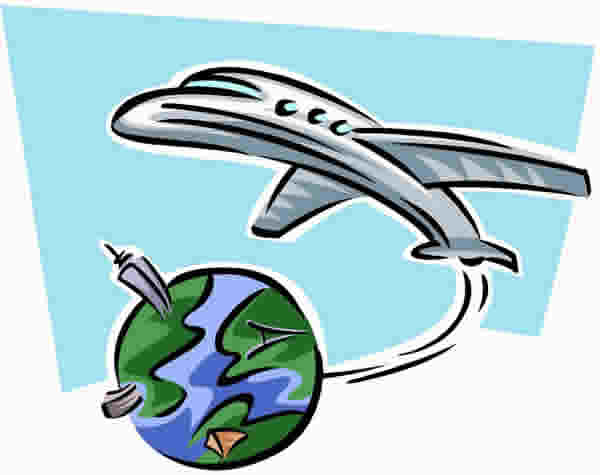
\includegraphics[scale=0.45]{viaje}}
\author{\textsc{Grupo 3:}\\
	Enrique Ballesteros Horcajo\\
	Ignacio Iker Prado Rujas}
\date{\Today}
\maketitle

\newpage
\mbox{}
\thispagestyle{empty}						% Hoja en blanco, sin numeros ni nada
\newpage


\tableofcontents 							%INDICE hipervinculado

\newpage
\mbox{}
\thispagestyle{empty}						% Hoja en blanco, sin numeros ni nada
\newpage

\pagenumbering{arabic}						% Pone el contador de paginas a 1 y ahora en numeros normales

\vspace{3cm}


\newpage



\begin{section}{Diseño del prototipo}

	\begin{subsection}{Identificar todos los conceptos que van a ser utilizados por el sistema.}

		\begin{itemize}
			\item Precio medio
			\item Monumentos
			\item Habitantes			
			\item Hoteles
			\item Albergues
			\item Campings
			\item Montaña
			\item Playa
			\item Parque de atracciones
			\item Discoteca
			\item Coche
			\item Avión
			\item Autobús
			\item Tren
			\item Deporte (Aventura, extremos, naturaleza)
			\item Balnearios
			\item Museos
			\item Operas
			\item Restaurantes
			\item Acceso discapacitados
			\item Destino
			\item Fácil llegada
			\item Intereses (Relax,  turismo, aventura, ...)
			\item Medio transporte
			\item Alojamiento
			\item Nombre
			\item Edad
			\item Personas
			\item Niños
			\item Presupuesto
			\item Discapacidad



		\end{itemize}

	 Por ejemplo: destino, transporte, alojamiento, hotel, apartamento, centros comerciales, 
	discotecas, restaurantes, museos, tipos de destino (cultura, descanso, ocio nocturno, 
	aventura, niños,...), nombre del	usuario, edad, gustos, restricciones, presupuesto disponible, etc.

	\end{subsection}

	\begin{subsection}{Identificar las relaciones existentes entre los conceptos}
	
	Por ejemplo: hotel es un tipo de alojamiento, Mallorca es un destino de playa,
	 los usuarios tienen nombre, edad, gustos, presupuesto, etc.).

		\begin{itemize}
			\item Un hotel es un alojamiento.
			\item 
			\item 
			\item 
			\item 
			\item 
			\item 
			\item 
			\item 
			\item 

			\item 

			
		\end{itemize}
	\end{subsection}

	\begin{subsection}{Dividir el problema en subproblemas o fases de funcionamiento del sistema.}
		
	 Para cada uno de estos subproblemas o fases, expresar con palabras todas las reglas que 
	van a ser utilizadas en su resolución.

	\end{subsection}


	
\end{section}
	\newpage
	\begin{section}{Prototipo}

		Implementar en Jess el conocimiento identificado en la primera parte. Cada subproblema o
		fase se implementará en un módulo distinto.


		Probar el prototipo con distintos conjuntos de datos. Los resultados obtenidos se incluirán
		también en la memoria, analizando su validez y proponiendo posibles mejoras.

	\end{section}

	
\begin{thebibliography}{9}

\bibitem{aima}
	Russell, S.; Norvig, P, \\
	\emph{Artificial Intelligence, a modern aproach}.\\
	New Jersey: Pearson, 2010.
	
\bibitem{clase}
	Apuntes y transparencias de Inteligencia Artificial, \\
	Doble Grado Matemáticas - Ing. Informática, U.C.M., 2014-2015.

\end{thebibliography}


\end{document}